% Copyright (c) 2007, Tobias Wolf <twolf@access.unizh.ch>
% All rights reserved.  

%
% Kapiteldatei
%


\chapter{Zusammenfassung}
\label{conclusion}

Diese Semesterarbeit hatte zwei Ziele. Zum ersten die Umsetzung einer neuen 
Datenstruktur f�r die effiziente Verwaltung von polygonalen Daten, und zum 
zweiten ein ebenfalls effizientes aber auch optisch ansprechendes Rendering 
dieser Daten.

Der erste Teil der Arbeit wurde vollst�ndig umgesetzt, die Implementierung der
neuen kd-Tree Datenstruktur erf�llt s�mtliche in Abschnitt \ref{requirements} 
gestellten Anforderungen. Der einzige sp�rbare Nachteil im Vergleich zur alten
Datenstruktur ist ein bedeutend langsamerer Aufbau des Baumes. Da nach der
erstmaligen Erstellung aber sowieso bin�re Repr�sentationen gespeichert werden
und f�r weitere Aufrufe verf�gbar sind, ist dieser Punkt vernachl�ssigbar. Der
Speicherverbrauch wurde auf weniger als ein Viertel reduziert (siehe Tabelle
\ref{tbl:file-sizes}).

Momentan wird der kd-Tree von jedem Renderknoten vollst�ndig geladen. Eine
denkbare Erweitung f�r die Verwendung mit der Equalizer DB Dekomposition w�re
beispielsweise, ein teilweises Laden nur der ben�tigen Bereiche zu erm�glichen.
Die Effizienz des View Frustum Cullings liesse sich unter Umst�nden verbessern,
indem statt beim Aufbau die Sortierachse zu rotieren jeweils diejenige mit der
l�ngsten Dimension gew�hlt w�rde. 

Des weiteren steht die Ausgliederung der Mesh Klassen in eine eigenst�nde 
Biobliothek aus, um diese auch f�r andere Projekte verwenden zu k�nnen. Als 
Folge daraus w�re auch eine GLUT Applikation denkbar, welche die Benutzung 
der Mesh Klassen in einer stand-alone Umgebung demonstriert.

Der zweite Teil der Arbeit erreicht die definierten Ziele teilweise. Das neue
Rendering mit Vertex Buffers Objects ist implementiert und funktioniert. Auch
Rendering mit Display Listen wird als OpenGL 1.1 kompatible L�sung weiterhin 
angeboten, und bleibt zur Zeit noch die Standardeinstellung. VBO Verwendung
kann �ber einen Kommandozeilenparameter aktiviert werden.

Ein Vergleich der Renderingperformance zwischen der alten und der neuen 
Applikation findet sich in folgender Tabelle \ref{tbl:render-performance}. 
In einigen F�llen bleibt die VBO Performance aus bisher ungekl�rten Gr�nden 
hinter den Erwartungen zur�ck, w�hrend sie in anderen F�llen einen markanten
Leistungsvorteil zeigt. Die verwendeten Modelle stammen aus 
\cite{stanford:repository} und \cite{cyberware}.

\begin{table}[ht]
\centering
\begin{tabular}{lrrrr}
\textbf{Modell} & \textbf{Anzahl} & \textbf{eqPly (alt)} & 
\textbf{eqPly (neu)} & \textbf{eqPly (neu)}\\
\textbf{} & \textbf{Triangles} & \textbf{DL [FPS]} & 
\textbf{DL [FPS]} & \textbf{VBO [FPS]} \\
Stanford Bunny   &      69'451  &  406.82   &   436.67   &   617.00\\
Rocker Arm       &      80'354  &  445.61   &   445.57   &   301.67\\
Goddess 1        &     274'822  &  142.20   &   162.45   &    70.94\\
Armadillo        &     345'944  &  118.30   &   136.43   &    92.17\\
Ganesh           &     413'236  &           &            &         \\
Boat             &     776'374  &   29.25   &    20.06   &    28.47\\
Dragon           &     871'414  &   17.06   &    45.02   &    38.19\\
Goddess 2        &   1'047'330  &   10.02   &     9.32   &    42.99\\
Hip              &   1'060'346  &   11.10   &     9.24   &    29.37\\
Happy Buddha     &   1'087'716  &    9.54   &    29.27   &    34.88\\
Asian Dragon     &   7'219'045  &           &            &         \\
Thai Statue      &  10'000'000  &           &            &         \\
\end{tabular}
\caption{Vergleich Renderingperformance altes und neues eqPly}
\label{tbl:render-performance}
\end{table}

Das Rendering ist durch die standardm�ssige Nutzung von Gouraud anstelle 
von Flat Shading bereits optisch deutlich ansprechender als in der alten 
Applikation. Dies ist in Abbildungen \ref{fig:sample-flat} und 
\ref{fig:sample-smooth} am Beispiel des RockerArm Modells zu sehen. 

\begin{figure}[hb]
\centering
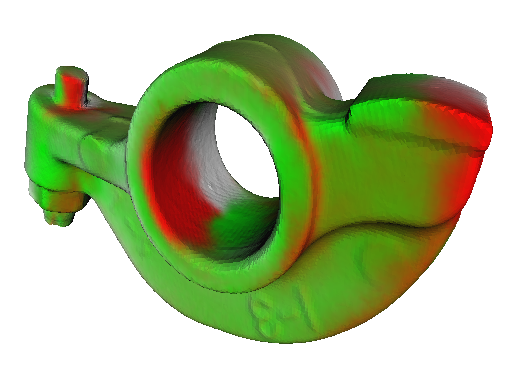
\includegraphics[width=0.86\textwidth]{figures/FlatShading.png}
\caption{RockerArm Modell mit Flat Shading}
\label{fig:sample-flat}
\end{figure}

\begin{figure}[ht]
\centering
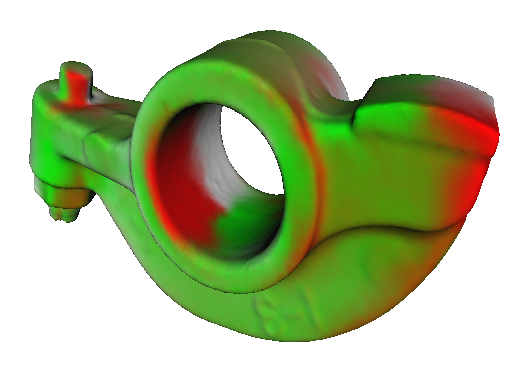
\includegraphics[width=0.86\textwidth]{figures/SmoothShading.png}
\caption{RockerArm Modell mit Gouraud Shading}
\label{fig:sample-smooth}
\end{figure}

Der Einsatz von GLSL Shadern und Phong Shading verbessert dies je nach Licht- 
und Materialeigenschaften noch einmal. Weitere Algorithmen konnten aufgrund 
mangelnder Zeit leider nicht mehr realisiert werden, das vorhandene Ger�st 
sollte das Hinzuf�gen weiterer Shader Algorithmen zu einem sp�teren Zeitpunkt 
jedoch problemlos erm�glichen.


%
% EOF
%
